%\documentclass{article}
%\documentclass[11pt]{article}   % Preset settings for two columns

\documentclass{llncs}

%\setlength{\textheight}{9.0in}
%\setlength{\textwidth}{6.5in}
%\setlength{\columnsep}{0.375in}
%\setlength{\oddsidemargin}{0.0in}
%\setlength{\topmargin}{0.0in}
%\setlength{\headheight}{0.0in}
%\setlength{\headsep}{0.0in}
%\setlength{\parindent}{1pc}

%\usepackage{doublespace}

\usepackage[pagewise]{lineno}       % For line number
\linenumbers

\usepackage{alltt}                         % For program with subscript
\usepackage[mathcal]{euscript}             % For special math symbol

\usepackage{graphicx}                      % For EPS figure
\usepackage{times}                         % For PDF font

%\usepackage{hyperref}                      % For hyper link, should be the last one 

\usepackage[ruled, vlined]{algorithm2e}    % For algorithm, 
                                           % it seems a bug make it has to be here

%\usepackage{epsfig}                        % For old PS figure

%\pagestyle{empty}                         % No page Numbering
\pagestyle{plain}                         

%%%% Define theorem
%\newtheorem{theorem}{Theorem}[section]

%------------------------------------------------------------------------- 
%------------------------------------------------------------------------- 

\begin{document}

%--------------------

% title.tex

\date{\today}      %%%% so that date does not print.

\title{Busy-wait barrier synchronization using distributed counters with local sensor}

\author{Guansong Zhang, 
Francisco Martinez\thanks{Ph.D. candidate, research student visiting from the Technical University of Catalonia (UPC), Barcelona, Spain},\\ 
Arie Tal, Bob Blainey} 

\institute{IBM Toronto Lab \\ 
Toronto \\ 
ON, L6G 1C7, Canada}

\maketitle

\thispagestyle{empty}

% abstract.tex

\noindent  
\emph{Abstract:} { Although OpenMP has become the leading standard in
  parallel programming languages, the implementation of its runtime
  environment is not well discussed in the literature. In this paper,
  we introduce some of the key data structures required to implement
  OpenMP workshares in our runtime library and also discuss
  considerations on how to improve its performance.  This includes
  items such as how to set up a workshare control block queue, how to
  initialize the data within a control block, how to improve barrier
  performance and how to handle implicit barrier and nowait
  situations. Finally, we discuss the performance of this
  implementation focusing on the EPCC benchmark.}

\vspace{0.5cm}

\noindent
\emph{Keywords:} {\small OpenMP, parallel region, workshare, barrier, nowait}



%--------------------

%%\pagebreak

\section{Thread mapping}

%What is mapping
The objective of \emph{thread mapping} or \emph{thread binding} is to define a
way to associate threads to physical processors. Once
mapped, the thread will stay on the processor during the execution without
being moved from one processor to another by the operating system. This is also
referred to as \emph{thread affinity}.

%Why mapping

A typical situation that needs thread mapping is shown in Figure
\ref{fig:mapping}, we have two dual core processors, each core is capable of
running two threads simultaneously. So the system can provide up to eight
\emph{physical threads} to an OpenMP application. 

In this system, suppose each processor core has its own L2 cache, and each CPU
core has its own L1 cache.

\begin{figure}[h!]
  \begin{center}
    \includegraphics[angle=0, width=0.45\textwidth]{mapping.eps}
    \caption{\footnotesize Thread mapping}
    \label{fig:mapping}
  \end{center}
\end{figure}

If an OpenMP application running on such system decides to use only four OpenMP
threads, then there are at least two mapping options one may choose from,

\begin{itemize} 

\item  let each CPU core have one OpenMP thread, so every processor core is
fully utilized. Or

\item let each CPU core have two OpenMP threads, leaving two CPUs idle. In this
way threads can share more data in cache among the adjacent ones.

\end{itemize}

It is hard to predict which mapping option can achieve better performance at an
abstract level. Depending on the hardware implementation and the program
itself, the answer may be different. So it will be desirable to let users
define the mapping to get better performance.

\subsection{Logical processors}

Before we define the actual mapping, it is important to think from an
application programmer's point of view, what kind of abstract view the hardware
system should look like.

A parallel program itself may be complicated enough that a regular user may not
want to know anything more than the number of processors offered in a system.
This is partially reflected in the current OpenMP standard. In \cite{Ope05}, an
API function \texttt{omp}\_\texttt{get}\_\\\texttt{num}\_\texttt{procs} returns
the number of the processors available to the program at the time the routine
is called. Most of the cases, it will be used to define the initial value for
the internal control variable \emph{nthreads-var}, which controls how many
threads are going to be created when a parallel region is encountered later on.

The environment variable \texttt{OMP\_NUM\_THREADS} and the API function
\texttt{omp\_set\_\\num\_threads} provide ways to change this control variable.
Yet in the current standard, there is no clear relationship between entities
represented by this control variable and the number returned from the function
\texttt{omp\_get\_num\_procs}, especially when the two values are different. 

The thread binding proposal we present here is to establish the affinity
relations between the \emph{OpenMP threads} controlled by the
\emph{nthreads-var} variable and the number of processors queried by
\texttt{omp\_get\_num\_procs}. In our proposal, we consider that the number
returned in the function \texttt{omp\_get\_num\_procs} is only for a
group of \emph{logical processors}. In Figure \ref{fig:mapping}, this number
can either be 4 or 8 depending whether the operating system made the extra
threads available. It is in contrast to the \emph{physical processors}, which
may be only 4 traditionally.

As an initial step, we will organize the logical processor group as a linear
array, giving each of them an id number, starting from 0, 1, and up to the
total number of the processors minus one.

Then the thread binding problem becomes the problem of having \emph{m}
OpenMP threads, and \emph{n} logical processor, how to assign those threads to
the processors, especially when $m \not= n$.

%Mapping define
\subsection{The mapping definition and its effect}

As explained above, we define the logical processors as a linear array. 

%We believe it is  
%enough complicated at this level that multi-dimension array is not needed. 

We use two environment variables to specify the first processor number that the
master thread binds to; and we specify the next processor number the second
thread will bind on with a "stride" on the processor array. 

For example, the following pair of environment variables

{\footnotesize
\begin{verbatim} 
    OMP_PROC_START=1; OMP_PROC_STRIDE=2
\end{verbatim}
}

will give us the mapping drawn in Figure \ref{fig:mapping}, where thread 0 is
on logical processor 1, thread 1 is on logical processor 3, and so on.  
We will use a \emph{round-robin} fashion to assign the other threads. 

%One way of
%defining it can be specified in the following pseudo code,

%{\footnotesize
%\begin{verbatim}
%    int num_Procs = omp_get_num_procs();
%    int num_Threads = omp_get_num_threads();
%
%    int start = getenv ("OMP_PROC_START");
%    int stride = getenv ("OMP_PROC_STRIDE");
%
%    int numPerRound = (num_Procs + stride -1 ) / stride;
%
%    for (int i = 0; i < num_Threads; i++) {
%      int round = i / numPerRound;
%      int count = i % numPerRound;
%
%      proc = (((start+round)+ stride * count)) % num_Procs;
%
%      // Assign thread i on processor proc
%      // This will be OS specific
%      ...
%    }
%\end{verbatim}
%}

%The round-robin method we used is always shifting one further from the start
%position in the previous round. Other alternatives are possible.

% Real example

\begin{figure}[h!]
  \begin{center}
    \includegraphics[angle=0, width=0.60\textwidth]{specomp.eps}
    \caption{\footnotesize SPEC OMP performance}
    \label{fig:specomp}
  \end{center}
\end{figure}

We used SPEC OpenMP benchmark to demonstrate the performance impact of thread
mapping. In Figure \ref{fig:specomp}, a 64 processor core POWER5 machine is used to
measure the OpenMP suite. The SMT option of POWER5 was on. So each processor is
capable of running two threads.  We set \texttt{OMP\_NUM\_THREADS} to be 64,
and compared the following situations

\begin{itemize}
    
  \item No processor mapping specification.

  \item Stride as one by \texttt{OMP\_PROC\_START=0; OMP\_PROC\_STRIDE=1}, and

  \item Stride as two by \texttt{OMP\_PROC\_START=0; OMP\_PROC\_STRIDE=2}

\end{itemize}

The rest of the execution environment, including compilation flags, are all the
same. From the figure, one can see that stride two setting has the best overall
performance numbers; Stride one setting is the worst: No stride setting is in
between.  And some of the difference can be as big as 40\%, such as in
equak, apsi and wupwise.


\subsection{More about the mapping}

In the mapping scheme above, all the processors and threads are kept in a
simple linear relation. More complicated mapping may be achieved though other
structures. For example, we can define a arbitrary mapping as an integer array.
We are not sure that such level of complexity is useful. We will see that more
complicated mapping actually can be achieved in the next section when we extend
the logical processor array to a \emph{processor group}.

We also need to point out that the mapping we defined here is only the one from
the OpenMP threads to the logical processors. We did not define how logical
processors mapped to physical threads. It is left as an implementation defined
issue. 

%For example, if the operating system is different, this mapping will be
%different.



%In our experiment, we have tested on AIX and Linux on POWER system.

%Even in this simple format
%Linux has special way of naming processors

%Merging two physical processors into one
%this is cell, extra thing needed? 
%at least access shared variable is complicated.

%As a summary, we did not involve nested parallelism and thread grouping in this
%first step.  Yet more complicated mapping options introduced in the next
%section will be considered as a natural extension of what we discussed here.




%%\newpage

\section{Overhead of a barrier synchronization}
\label{overhead}

There are many ways of implementing a barrier synchronization. In this
paper, we focus on the so-called \emph{centralized barrier}, simply
because in a globally addressed memory system with wide bandwidth
among node processors, such as a POWER4, the centralized barrier will
make the coding much easier, and less error prone\footnote {When there
  is a large number of processor nodes connected by a interconnection
  network with a specific topology, centralized barrier may not be
  preferable. While the barrier in Figure \ref{fig:barriers} (b) will
  be more interesting, where locality is emphasized.}.

Several ways to implement this kind of barrier were suggested in
\cite{Mel91} and re-examined on a ccNUMA system in \cite{Nik99}.
Basically, a shared variable is updated as each thread arrives at the
barrier point. The thread will leave the position if testing finds out
that all the threads have arrived. To understand the overhead of the
whole process, we first have a brief introduction on the 
hardware architecture used for testing, and our test
environment.

\subsection{POWER4 SMP architecture and software}

The basic building block for a POWER4 SMP system can be found in
\cite{Ste01}. It is a multi-chip module (MCM) with four POWER4 chips
forming an 8-way SMP, as shown in Figure \ref{fig:mcm}.  Multiple MCMs
can then be interconnected to form 16-, 24-, and 32-way SMPs.

\begin{figure*}[hbt]
  \begin{center}
    \includegraphics[angle=0, width=0.8\textwidth]{power4mcm.eps}
    \caption{POWER4 MCM structure}
    \label{fig:mcm}
  \end{center}
\end{figure*}

The logical interconnection of four POWER4 chips is point-to-point,
with uni-directional buses connecting each pair of chips to form an
8-way SMP with an all-to-all interconnection topology. The fabric
controller on each chip monitors (for example snoops) all buses and
writes to its own bus, arbitrating between the L2 cache, I/O
controller, and the L3 controller for the bus. Requests for data from
an L3 cache are snooped by each fabric controller to determine if it
has the data being requested in its L2 cache (in a suitable state), or
in its L3 cache, or in the memory attached to its L3 cache. If any one
of these is true, then that controller returns the requested data to
the requesting chip on its bus. The fabric controller that generated
the request then sees the response on that bus and accepts the data.

Up to four MCMs can be interconnected by extending each bus from
each module to its neighboring module in one direction. Inter-module
buses run at half the processor frequency and are 8-bytes wide. The
inter-MCM topology is that of a ring in which requests and data move
from one module to another module in one direction. As with the single
MCM configuration, each chip always sends requests, commands and data
on its own bus but snoops all buses for requests or commands from
other MCMs.

The underlying software system is the SMP runtime library supporting
the OpenMP standard. It is not a research system but production
level software available in the IBM$^{\textregistered}$ 
XL Fortran and VisualAge C++$^{\textregistered}$ products.
The runtime system implements schedule-based barrier synchronization
as well as a fallback for the busy-wait method.

\subsection{Testing benchmark}

We use unmodified EPCC micro-benchmarks to test the performance of a
barrier synchronization. As introduced in \cite{Bul99}, the overhead
here is considered as the difference between the parallel execution
time and the ideal time, given by perfect scaling of the sequential
program.

The parallel execution time is taken from the following code segment, 

%\begin{figure*}[htbp]
%  \begin{center}
{\small
\begin{verbatim}
      dl = delaylength

      do k=0,outerreps
         start  = getclock()
!$OMP PARALLEL  PRIVATE(J)                   
         do j=1,innerreps
            call delay(dl)
!$OMP BARRIER                                
         end do
!$OMP END PARALLEL
         time(k) = (getclock() - start) *
     &             1.0e6 / dble (innerreps)
      end do
\end{verbatim}
% close the $
}
%    \caption{EPCC barrier test}
%    \label{fig:epcctest}
%  \end{center}
%\end{figure*}

While the sequential reference time is measured through this code,

{\small
\begin{verbatim}
      dl = delaylength 
      do k=0,outerreps
         start  = getclock()
         do j=1,innerreps
            call delay(dl)
         end do
         time(k) = (getclock() - start)*
     &             1.0e6 / dble (innerreps) 
      end do
\end{verbatim}
}

In the test program, the value of \texttt{outerreps} is set to 50,
which is the default in the EPCC micro-benchmarks. The array variable
\texttt{time} is used to compute the mean and standard deviation of
the 50 measurements. Since we can exclusively access the machine, only
the mean value is considered here.

\subsection{Barrier overhead on an SMP system}

The two main reasons for the overhead of a barrier synchronization are
memory contention and traffic.  We define \emph{contention} as the effect
produced by many threads accessing simultaneously the same data, and
\emph{traffic} as the amount of data per time unit moving through the
bus. 

Nevertheless, contention and traffic are not independent as some
accesses to memory increase both (so, contention in one memory
position is likely to increase traffic).  Studying memory behavior
through hardware counters can show us an approximation to both the
contention and traffic that a concrete barrier implementation puts on
the system.

In order to reduce the complexity of the analysis, we separate the
barriers into phases:

\begin{itemize}
\item Signaling: Time to enter the barrier and notifying that we are
  in
\item Leaving: Time to realize that the synchronization is over and we
  can leave the barrier
\end{itemize}
This classification can be useful because some implementations focus on 
reducing the impact of the first while others focus on the second. 


%The overall overhead can be calculated, then, as the sum of
%those two times. Decomposition of the barrier in those two times can
%be interesting because in some cases behavior between the two phases
%is significantly different.




%\newpage

\section{Key data structures}
\label{design}

In this section, we will examine the techniques for implementing
workshares in a parallel region. 

%The data structures is explained in a ``top-down'' manner.
 
\subsection{General requirement}
\label{sec:require}

The specific ways of implementing workshares in a parallel region may
be different from one to another, but with the analysis we already
have in previous sections, one can see that at least the following
data segments should be in a \emph{control block} for workshares,

\begin{itemize}
\item \emph{Structure to hold workshare-specific information} This is
  needed to store information regarding an OpenMP DO construct or
  SECTIONS construct. Things like initial, final value of the loop
  induction variable, the schedule type, etc.
\item \emph{Structure to complete possible barrier synchronization}
  This is used to implement any barriers that may be needed during the
  lifetime of the workshare construct.
\item \emph{Structure to control access to the workshare control
    block} This is typically a \emph{lock} to ensure only one thread
  modifies the information of the shared control block, for example,
  to mark the workshare started or show that a particular section code is
  already done.
\end{itemize}

Since different workshare constructs can be put into the same parallel
region, the first item must be a ``\emph{per workshare}'' value, i.e.
for each workshare in the parallel region, there should be a
corresponding one. Because of the existence of NOWAIT clauses,
multiple workshares can be \emph{active} at the same time --- executed
by different threads simultaneously.  So, multiple instance of this
data structure must exist simultaneously; one for each active
workshare. The same observation can be made for the third item in the
list. Each thread will access its own active workshare control block,
which may or may not be different from each other.

%Discussion on the second item is out of the interest in this note, for
%general structures to implement a barrier synchronization, please
%refer to \cite{Mel91}.

In general, there has to be a queue of workshare control blocks for
each parallel region.

\subsection{The control block queue length}
\label{sec:size}

Once we understand the basic structures needed for a parallel region,
we have to consider its construction, destruction and initialization.
At the same time, we need to minimize the overhead of creating and
manipulating such structures, as noted in \cite{Bul99}.

It cannot be statically predicted how many parallel regions a program
may explore and how many of them will be active at the same time because 
of nested parallelism or explicit usage of threads in user codes.
Therefore, the workshare control block queue will be allocated
dynamically. In addition to discussions in section \ref{sec:require}, a
workshare control block queue has to be constructed whenever a
parallel region is encountered, and it will be destroyed when the
parallel region ends.

Before we go any further, we need to decide the length of this queue.
For example, if we map each workshare to its own control block
in a straightforward manner, the following parallel region

{\small
\begin{verbatim}
      !$OMP PARALLEL 
      !$OMP DO
            DO i = istart, iend
              ...
            END DO
      !$OMP END DO
      !$OMP DO
            DO i = istart, iend
            ...
            END DO 
      !$OMP END DO NOWAIT
      !$OMP DO
            DO i = istart, iend
            ...
            END DO
      !$OMP END DO
      !$OMP DO
            DO i = istart, iend
            ...
            END DO
      !$OMP END DO
      !$OMP END PARALLEL
\end{verbatim}
}

will need the workshare control block queue as shown in Figure
\ref{fig:queue}, where there are four block elements in total.

\begin{figure}[!h]
  \begin{center}
    \includegraphics[angle=0, width=0.7\textwidth]{queue.eps}
    \caption{\footnotesize Workshare control block queue}
    \label{fig:queue}
  \end{center}
\end{figure}

A simple way of handling the queue is to create a new control block
whenever a workshare is encountered, more accurately, whenever a
\emph{workshare instance} is encountered. If a workshare is defined
inside a sequential loop body, we have as many workshare instances as
the number of iterations in that loop.

Since the workshare control block is a shared construct for multiple
threads, to constantly increase its size will be detrimental to the
runtime overhead for the creation of parallel regions. Moreover, doing so
will create higher memory impact on the overall program execution.

A better solution is to allocate a chunk of workshare control blocks
at once, use them as a block pool, and try to reuse the pool whenever 
possible, only increasing its size when absolutely necessary.

In the queue, we will set up extra fields, such as \emph{next
  available workshare control block pointer}, and set it back to the
beginning whenever an explicit or implicit barrier is met. Thus we
only need two block structures instead of the four in Figure
\ref{fig:queue} for the code snippet above. When the first workshare
instance finishes, a barrier synchronization occurs, and the next
available workshare control pointer will be set back to the first
block structure. Then, two block structures are needed at most because of
the NOWAIT clause. After that, another barrier will set the pointer
back to the beginning again.

%The length needed for the queue is actually the maximum number of
%active workshares in the parallel region. We can allocate a chunk of
%workshare control blocks as the initial pool, then with the method
%described above keep reusing it. This will also help to improve the
%cache locality of the program. 

Furthermore, resizing the pool may need extra book-keeping structures
and work. If we artificially introduce a barrier on a nowait workshare
when the queue becomes full, we do not need to increase the size at
all\footnote{We do need to mark the head and tail position of the
active workshares in the queue, so the next available pointer can be
set, from the position next to the head, back to its tail when a
barrier is encountered.}.

In real applications, a special case of using of NOWAIT clauses is to
form a coarse-grain software pipeline, such as the one in APPLU of
SPECOMP2001\cite{Spe01}, thus one cannot degrade any nowait
workshare. But in such cases, the length of the pipeline is often set
as the number of the hardware processors to get best performance.
Choosing a proper fixed-size queue to avoid extra overhead is still a
valid consideration.

Regardless of resizing the queue or not, the number of hardware
processors or its multiples, to be conservative, is a good candidate
for the initial chunk size of the pool. Then we can resize the queue
if needed.

\subsection{Fine-grained optimization}
\label{sec:optimize}

From the analysis in section \ref{sec:require}, a lock has to be defined
within the control block structure. Whether it is hand coded as in
\cite{Mel91} or used directly from Pthread library\cite{But97}, the
lock itself needs to be initialized, along with other structures for
the workshare-specific information.

The master thread can initialize all the structures at once when they
are allocated during the setup time. But for parallel regions where
the maximum number of active workshares is small --- only one, when
the NOWAIT clause does not exist, this process will bring extra overhead.
It is more desirable to defer the initialization of the block items
until their use becomes necessary.

Algorithm \ref{alg:workshare}, used to execute a workshare, achieved
this by always keeping the queue have one extra block ready during
initialization phase. In the scheme, the master thread initializes the
first control block, thus making the queue ready to use for the first
workshare. Then, when the first thread exclusively accesses the
available control block through the lock, it will make the next
control block available by initializing it.

%A counter may be used to indicate how many blocks have been
%initialized. 

\begin{algorithm}[h]
  \SetLine %this is vertical line
{\small
  \AlgData{Workshare control block queue}
%    allocated and with its first element initialized by the master thread}
  \AlgData{Next available block pointer}
  \BlankLine

  \Begin {
    \If{this workshare is not locked} {
      lock it\;
      \eIf {this workshare is already started} {
        release the lock\;
      } {
        mark this workshare has been started\;
        init the next available control block if it is new\;
      }
    } 
    execute the corresponding workshare and 
    release the lock if I have locked it\;
    \If {barrier is needed} {
      do barrier synchronization and
      reset the next available control block pointer\;
    }
  }
}
  \caption{Execute a workshare in parallel regions}
  \label{alg:workshare}
\end{algorithm}

The next control block may never be used. But by keeping it ready, we
do not need another lock process to initialize a shared item. The lock
is shared with the exclusive access to the previous control block.
The exclusive access here is needed anyway, since each thread needs
to know if the workshare has been worked on.

\subsection{Barrier implementation}
\label{sec:barrier}

There are many papers dedicated to the implementation of a barrier synchronization
already. Here we will use
Algorithm \ref{alg:barrier} described in \cite{Zha03}.


%\footnote{Note that we did not emphasize the data structure
%  here, they can be either a padded one or not, or even share the same
%  cache line as we discussed previously.}.

\begin{algorithm}[h]
  \SetLine
{\small
  \AlgData{Distributed counter with each element as one}
  \AlgData{Local sensor with each element as one}
  \BlankLine
  \Begin {
    Decrease my own distributed counter element\;
    \eIf{I am the master thread}{
      \Repeat{all distributed counter elements are zero} {
        \lForEach{element in distributed counter}{check if it is zero}
      }
      \ForEach{element in distributed counter}{set it back to one}
      \ForEach{element in local sensor}{set it to zero}
    }{
      \Repeat{it is zero} {
        check my local sensor element
      }
    }
    Set my own local sensor element back to one\;
  }
}
  \caption{Barrier with distributed counter and local sensor}
  \label{alg:barrier}
\end{algorithm}


Since both distributed counter and local sensor are padded cachelines,
we would like to avoid allocating two cache line arrays for every
barrier by letting all the barriers in a parallel region share the
same pair of counter and sensor.

Before a barrier starts, all the elements of the counter array will be
set to one, as will the local sensor counter array. We let one thread
in the group, for instance the master thread, act as if it is the last
thread. It will decrease its own element of the distributed counter
array and then spin to check whether all of the counter elements are
zero. The rest of the threads will decrease their own counter elements
and then spin on checking their own local sensors.

When the designated thread finds the counter elements are all zero, it
will set all the counter elements back to one and then zero all of the
elements in the local sensor array.  Finally, when all of the threads
leave the barrier after their local sensor is zeroed, they reset their
local sensor back to one.

%\subsection{Summary of claims}
%\label{sec:claim}

%We summarize the related claims as following,

%\begin{itemize}
%\item Structures to implement workshares, including the workshare
%  control block queue and the next available pointer
%\item Algorithm to execute different kinds of workshares, including
%  OMP DO, SECTIONS, SINGLE constructs and the explicit barrier.
%\item Scheme to reuse workshare control block queue.
%\item Initialization of the workshare control block queue, to make the
%  next block available by the first arrived thread.
%\end{itemize}

%Through these structures and algorithms, we think we have an optimized
%frame work for implementing OpenMP workshares.


%\section{Other techniques and performance gain}


We used the EPCC microbenchmarks\cite{Bul99} to show the performance
gains coming from optimization considerations we discussed in previous
sections. The hardware systems we tested on are a 16-way 375MHz
POWER3$^{TM}$ and a 32-way 1.1GHz POWER4$^{TM}$.

The EPCC benchmarks have two parts, the synchronization suite and the
schedule suite. Since we are concentrating on workshare
implementation, we have focused on the synchronization benchmark. It
includes separate test cases for parallel region, workshares (which are
OMP DO, SINGLE and explicit barrier), and reductions.

For a parallel region, as we show in Figure \ref{fig:compare}, the ``on
demand'' initialization method introduced in section
\ref{sec:optimize} reduces its overhead on both POWER3 and POWER4
systems. 

%This is the actual improvement we had over XL Fortran 8.1 and C/C++
%6.0.

\begin{figure}[!h]
  \begin{center}
    \includegraphics[angle=0, width=0.60\textwidth]{compare.eps}
    \caption{\footnotesize Performance difference}
    \label{fig:compare}
  \end{center}
\end{figure}

For a barrier operation, we compare a primitive fetch-and-add barrier
with the one using algorithm \ref{alg:barrier} and the results are
shown in Figure \ref{fig:power4performance}. The test was done on the
POWER4 system. As the number of threads increases, the advantage of
using distributed counters becomes more apparent.

\begin{figure}[!h]
  \begin{center}
    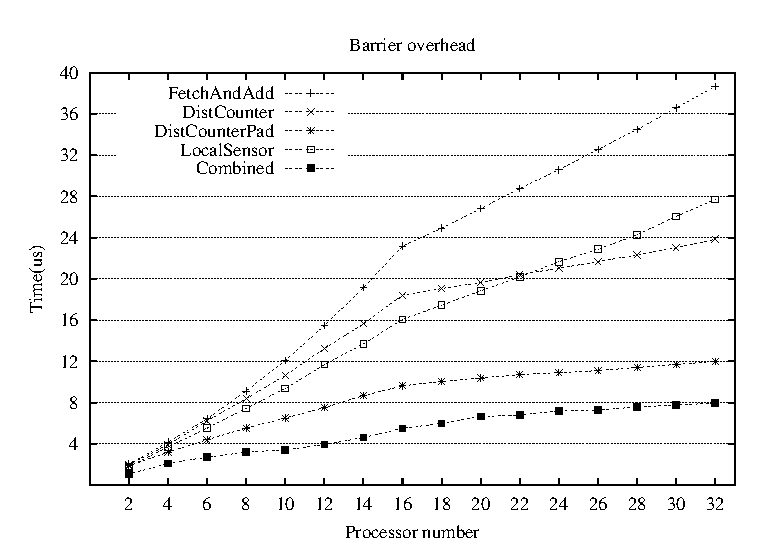
\includegraphics[angle=0, width=0.60\textwidth]{power4performance.eps}
    \caption{\footnotesize POWER4 barrier overhead}
    \label{fig:power4performance}
  \end{center}
\end{figure}

In fact, the whole sub-suite improved significantly with the methods
introduced in the previous sections. Again the data in Figure
\ref{fig:epcc} was collected on the POWER4 system.

\begin{figure}[!h]
  \begin{center}
    \includegraphics[angle=0, width=0.80\textwidth]{epcc.eps}
    \caption{\footnotesize EPCC improvement}
    \label{fig:epcc}
  \end{center}
\end{figure}

Note that in this figure, the reduction case is special; aside from
the improvement from a better parallel region and synchronization
method, we have also implemented a partial-sum mechanism to implement
the reduction, which allows us to minimize the required
synchronization.

% Both tests uses 16 threads.

%{\small
%\begin{verbatim}
%      dl = delaylength

%      do k=0,outerreps
%         start  = getclock()
%         do j=1,innerreps
%!$OMP PARALLEL
%            call delay(dl)
%!$OMP END PARALLEL
%         end do
%         time(k) = (getclock() - start) * 
%     &       1.0e6 / dble (innerreps)
%      end do
%\end{verbatim}
%}

%\emph{[More to be added, including complete EPCC results and analysis ... ]}


%%\newpage

\section{Summary and future work}
\label{summary}

Barrier synchronization is a well-studied topic, and an important
one in parallel programming. In this paper, we studied the performance
characteristics of several alternative implementations of barrier
synchronization on modern, complex shared memory multiprocessors.

We have implemented several different barrier schemes and measured their performance on the shared memory POWER3 system and the distributed shared
memory POWER4 system. We analyzed barrier performance data through
timing and hardware performance counters. In the future, we wish to study
the impact of different barrier implementations on other shared memory
platforms particularly looking at issues of non-uniform memory access and
scalability.

Through the introduction of the \emph{distributed counters with local sensor}
implementation, we have demonstrated a dramatic 79\% reduction in overhead on a
32-way POWER4 system when comparing to a fetch-and-add implementation and a 33\%
improvement on the same system over the next best technique, distributed
counters with padding.  While these experiments were done using the explicit 
barrier test in EPCC microbenchmarks,
we get similar improvements in the performance of the implied barriers
terminating work-sharing constructs and parallel regions.  The availability of
a low overhead barrier also provides more freedom to the compiler to automatically
introduce parallelism in serial code.

% how about irregular

%Understanding more about the ccNUMA system

%We treat the system more like a distributed message-passing one.

%memory affinity processor affinity.


%%\section{Acknowledgments}

\section{Trademarks and copyright}

AIX, IBM, POWER3, POWER4, and VisualAge are trademarks or registered
trademarks of International Business Machines Corporation in the
United States, other countries, or both.

\noindent Other company, product and service names may be trademarks or service
marks of others.
  

\noindent \copyright\ Copyright IBM Corp. 2004.  All rights reserved.





%--------------------

\bibliographystyle{unsrt}
\bibliography{permutation}

%--------------------

\end{document}

%------------------------------------------------------------------------- 
To do list
%------------------------------------------------------------------------- 

